To be able to carry out the simulation methods in a realistic way, most parts of the models are based on data collected from sources online, conversations with the Assistant Duty Manager at Avinor, Marit Kristoffersen \cite{marit} and information given in the assignment. However, some parts are based on subjective assumptions which will be explained in further detail in the following section. 

\section{Data from the Assignment}
\subsection{Airplane Configuration}
Data regarding initial model parameters have been collected from information given in the assignment. This involves an airplane configuration consisting of 20 rows, 6 seats per row and 1 aisle. The plane occupancy is always 100\%, which means that 120 passengers are boarding the plane.

\subsection{Time Measures}
The time it takes for a passenger to walk from one row to the next is based on a triangular distribution measured in seconds, where {min; mode; max} = {1.8; 2.4; 3}. The time it takes for a passenger to sit without interference is also triangular distributed, measured in seconds, where {min; mode; max} = {6; 8; 10}. An important factor in the simulation is the time it takes a passenger to store luggage, and is based on the following formula:
\begin{figure}[H]
\centering
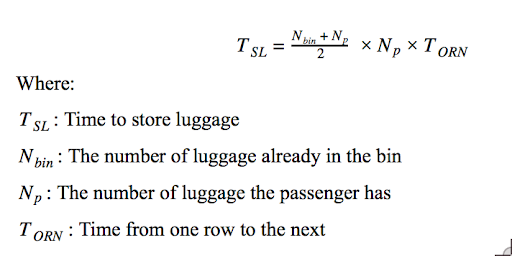
\includegraphics [scale=0.42,angle=360]{figures/unnamed.png}
\label{fig:unnamed}
\end{figure}
These criteria were incorporated into the models by changing the passengers’ speed according to the distance between the two consecutive rows, in case (1), and the distance between the center of the aisle and a middle seat, in case (2).

\section{Data from other Sources}
\subsection{Passengers Walking Speed}
People's average walking pace depends on the age of the person. Research has shown a speed ranging from approximately 1 meters/second to 1.5 meters/second \cite{speed}. Passengers in the model have therefore been set with a comfortable speed through a uniform distribution measured in meters per second, where {min; max} = {1.0; 1.5}. The speed applies only for situations where the passengers are able to walk uninterrupted. How fast passengers are moving in the aisle inside of the airplane is based on the time from one row to the next and the distance between two rows. The speed was calculated with a triangular distribution measured in meters per second, where {min; mode; max} = {0.94; 1.17; 1.56}. 

\subsection{Hand Luggage per Passenger}
There are different policies regarding the amount of hand luggage passengers are allowed to carry with them on an airplane. Searching the biggest airline's policies shows that it is common either to allow for 1 cabin bag + 1 personal item (laptop/handbag) or just 1 cabin bag \cite{luggage}. Based on this information, the simulation methods allow for passengers carrying up to 2 items of hand luggage.   

\subsection{Bin Capacity}
Based on personal experience, a common problem in the boarding process is the lack of space in the airplane bins, especially in situations where the airplane is fully occupied. One of the authors has a family member (Marit Kristoffersen) who has for many years worked in different roles at Oslo Airport, Gardermoen, and is currently working as an Assistant Duty Manager for Avinor. She was contacted in order to verify the assumption. She explained that this is a common issue among the airlines and an important factor to the boarding time. Hence, the simulation models consider a bin occupancy of 100%. 

\subsection{Data Sets}
In order to optimize the input of data used in the models and to make the scenarios easier to manage, data sets were created in excel and imported into the models. The data sets contain the values for various parameters used in the simulations. 